\section{Theorie}
\label{sec:Theorie}
Ziel des Versuchs ist es, das effektive Saugvermögen einer Drehschieberpumpe und einer Turbomolekularpumpe, zu bestimmen.
Dies geschieht zum Einen über die Evakuierungskurve und zum Anderen über eine Leckratenmessung.
Zudem sollen die Grundlagen der Vakuumphysik erlernt werden.


\subsection{Grundlagen}
\label{sec:Grundlagen}
Vakuum ist definiert als Druck, der geringer ist als der Erdatmosphärendruck auf der Erdoberfläche.
Dies ist in etwa bei $300 mbar$ (auf dem Mount Everest) der Fall \cite{Pfeiffer, S.9}.
Es gibt verschiedene Abstufungen von Vakuum. Diese reichen vom Grobvakuum bei $300 mbar - 1 mbar$, bis zum 
extrem hohen Vakuum bei Drücken von weniger als $10^{-12} mbar$ \cite{Pfeiffer, S.10}.
Druck, über den das Vakuum definiert ist, beschreibt die senkrecht auf eine Fläche wirkende Kraft, also $p = \frac{F}{A}$.
Um das Verhalten des Gases bzw. der Teilchen im Vakuum besser beschreiben zu können, wird dieses Gas als Ideales Gas angenommen.
Bei idealem Gas werden die Gasteilchen als punktförmige Massen ohne Ausdehnung beschrieben. 
Die Wechselwirkungen zwischen den Teilchen werden vernachlässigt, vorallem Van-der-Waals- und Dipol-Dipol-Kräfte.
Zudem wird angenommen, dass dei Teilchen ausschließich elastisch mit anderen Gasteilchen und den Wänden stoßen.
Wenn diese drei Annahmen gelten, ist das Produkt aus Druck und Volumen, bei konstanter Temperatur, konstant, 

    \begin{equation}
    \label{equ:0}
        pV = const 
    \end{equation}
so wie der Druck, in einem konstanten Volumen, proportional zur Temperatur, $p = const \cdot T$.
Daraus gergibt sich die Ideale Gasgleichung,

    \begin{equation}
    \label{equ:1}
        pV = N \cdot k_B \cdot T.
    \end{equation}
Dabei ist $N$ die Teilchenanzahl und $k_B$ die Boltzmann-Konstante.
Diese Gleichung kann als Ausdruck für den Druck in Abhängigkeit von der Teilchenzahldichte $n$ geschrieben werden, 
denn $n = \frac{N}{V}$.
Daraus folgt,

    \begin{equation}
    \label{equ:2}
        p = n \cdot k \cdot T.
    \end{equation}
Also ist die Teilchenzahldichte ein gutes Maß für den Druck und kann zur beschreibung des Drucks verwendet werden \cite{Pfeiffer, S.11}.
Ebenfalls eng mit der Teilchenzahldichte und damit dem Druck verknüpft und relevant für die Vakuumtechnik ist die mittlere freie Weglänge.
Diese beschreibt die durchschnittliche Länge des Weges, eines Teilchens, bis es mit einem anderen Teilchen oder einer Wand zusammenstößt 
und ist gegeben als,

\begin{equation}
\label{equ:3}
    \bar{l} = \frac{k \cdot T}{\sqrt{2} \cdot \pi \cdot p \cdot d_m^2}.
\end{equation}
Mit dem Moleküldurchmesser $d_m^2$ \cite{Pfeiffer, S.12}.


\subsection{Strömungen}
\label{sec:Strömungen}
Im Vakuum gibt es zwei wesentliche Arten von Strömungen, zum einen die viskosen Strömungen und zum anderen die molekularen Strömungen.
Eine Kennzahl zur unterscheidung der Strömungen ist die Knudsenzahl $K_n = \frac{\bar{l}}{d}$, also das Verhältnis zwischen mittlerer freier Weglänge 
und Weite des Strömungskanals.
Bei einer Knudsenzahl von $K_n < 0,01$ ist die Strömung viskos, bei $K_n > 0,5$ ist die Strömung Laminar. Zwischen den beiden Grenzen befindet sich die 
Knudsenströmung.
Die viskose Strömung zeichnet sich dadurch aus, dass die Gasteilchen hauptsächlich untereinander Stöße ausführen und kaum mit den Wänden.
In diesem Bereich gibt es zum einen die turbolente Strömung, bei der die Gasteilchen völlig ungeordnet sind. Diese Strömung tritt bei schnelleren 
Strömungsgeschwindigkeiten auf und ist im Vakuum nur beim Abpumpen von Atmosphärendruck und beim Belüften relevant.
Zum anderen gibt es die Laminare Strömung, bei der sich die Gasteilchen innerhalb parallel zueinander geordneten Schichten aufhalten.
Dies geschieht bei langsameren Strömungsgeschwindigkeiten der viskosen Strömung.
Die Molekulare Strömung ist vorallem im hochvakuum und ultra hoch Vakuum von bedeutung, da bei einer so geringen Teilchenzahldichte, kaum Stöße mit anderen Teilchen erfogen, 
sondern hauptsächlich mit Wänden \cite{Pfeiffer}.


\subsection{Saugvermögen, Leitwert}
\label{sec:Saugvermögen}
            %Aus der idealen Gasgleichung kann der kann ein Maß für den Gasstrom gewonnen werden, indem die Gleichung urch die Zeit $t$ dividiert wird,
            %
            %    \begin{equation}
            %    \label{equ:4}
            %        \frac{pV}{t} = \frac{n k T}{t}.
            %    \end{equation}
            %
            %Für eine Vakuumpumpe wird der Gasstrom auch Saugleistung genannt 
            %
            %    \begin{equation}
            %    \label{equ:5}
            %        q_{pV} = \frac{dV}{dt} p = S \cdot p.
            %    \end{equation}
            %
            %Darüber wird das Saugvermögen $S = \frac{dV}{dt}$ einer Vakuumpumpe definiert, also das pro Zeit abgepumpte Gasvolumen \cite{Pfeiffer, S.15}.
Das Saugvermögen einer Vakuumpumpe gibt an, wie viel Gas sie pro Zeit aus dem Rezipienten saugen kann,

    \begin{equation}
    \label{equ:4}
        S = \frac{dV}{dt}.
    \end{equation}
Die Rohre und Behälter in der Vakuumtechnik haben ähnlich wie elektrische Leiter, einen Widerstand.
Dieser Widerstand ist über die Druckdifferenz zwischen Ende und Anfang des Rohres und dem Gasstrom definiert,

    \begin{equation}
    \label{equ:5}
        W = \frac{\Delta p}{q_{pV}}.
    \end{equation}
Der Kehrwert des Widerstands wird Leitwert genannt und ist ein Maß dafür wie gut der Gasstrom durch ein Gefäß fließen kann,

    \begin{equation}
    \label{equ:6}
        L = \frac{1}{W} = \frac{q_{pV}}{\Delta p}.
    \end{equation}
            %Der Leitwert verhält sich bei Reihen- bzw. Parallelschaltung wie der Kehrwert des elektrischen Widerstands.
            %Für die Reihenschaltung gilt,
            %
            %    \begin{equation}
            %    \label{equ:7}
            %        \frac{1}{L_{ges}} = \frac{1}{L_{1} + \frac{1}{L_{2} + ...
            %    \end{equation}
            %
            %und für die Parallelschaltung \cite{Buch, S.80, 81},
            %
            %    \begin{equation}
            %    \label{equ:8}
            %        L_{ges} = L_1 + L_2 + ...
            %    \end{equation}
Aus diesem Rohrwiderstand ergibt sich, dass das Saugvermögen der Vakuumpumpe nicht dem theoretischen Wert entspricht, 
da die Pumpe normalerweise über einen Schlauch mit dem Rezipienten verbunden ist und dieser Schlauch aber auch der Rezipient selbst, 
einen Rohrwiderstand besitzen \cite{Buch, S82}.
Das Effektive Saugvermögen einer Vakuumpumpe ist daher,

    \begin{equation}
    \label{equ:9}
        S_{eff} = \frac{1}{S} + \frac{1}{L}.
    \end{equation}


\subsection{Evakuierungskurve}
Wird Gleichung \eqref{equ:0} nach der Zeit abgeleitet, 

    \begin{equation}
    \label{equ:10}
        \frac{dp}{dt} V + \frac{dV}{dt} = 0
    \end{equation}
und anschließend umgestellt, so entsteht ein Ausdruck für das Saugvermögen,

    \begin{equation}
    \label{equ:11}
        \frac{dV}{dt} = S = - \frac{V}{p} \frac{dp}{dt}.
    \end{equation}
Die Lösung dieser Differentialgleichung ist:

    \begin{equation}
    \label{equ:12}
        p(t) = p_0 exp \left(- \frac{S}{V}t \right)
    \end{equation}
Weiter muss beachtet werden, dass jede Vakuumpumpe einen Enddruck $P_E \neq 0$ erzeugt. 
Dies führt zur abschließenden Gleichung für die Evakuierungskurve:

    \begin{equation}
    \label{equ:13}
        p(t) = (p_0 - P_E) exp \left(- \frac{S}{V} t \right) + P_E.
    \end{equation}
Mit hilfe dieser Formel kann aus der Evakuierungskurve das Saugvermögen einer Vakuumpumpe bestimmt werden,
wobei hier nicht beachtet wurde, dass das Saugvermögen einer Vakuumpumpe nicht konstant über alle Drücke ist.


\subsection{Lecks}
Bei jedem Vakuumaufbau gibt es Lecks, die Verhindern, dass der Druck unter $P_E$ sinkt.
Es gibt zum einen reale Lecks, die von außerhalb der Vakuumanlage messbar sind, z.B. undichte Ventile 
aber auch "virtuelle" Lecks, bei denen das nicht der Fall ist.
Diese "virtuellen" Lecks werden z.B. durch \textbf{Desorption} verursacht.
Desorption beschreibt das Lösen/Austreten von Atomen oder Molekülen, von/aus einer Oberfläche.
Diese Atome und Moleküle sind vorher durch \textbf{Sorption} angelagert worden.
Bei der Sorption wird zwischen \textbf{Absorption}, also das in das Material rein diffundieren und \textbf{Adsorption}, 
dem Anlagern von Atomen und Molekülen an einer Oberfläche, unterschieden\cite{Buch, S.62,63}.


\subsection{Leckratenmessung}
Das Saugvermögen kann auch über die Leckratenmessung bestimmt werden.
Dafür muss zunächst eine Lecktrate $Q$ eingestellt werden, diese wird über den Gleichgewichtsdruck $P_g$ definiert,

    \begin{equation}
    \label{equ:14}
        S = \frac{Q}{P_g},
    \end{equation}
mit,

    \begin{equation}
    \label{equ:15}
        Q = V_0 \frac{\Delta p}{\Delta t}.
    \end{equation}
Aus Gleichung \eqref{equ:14} und \eqref{equ:15} folgt für das Saugvermögen:

    \begin{equation}
    \label{equ:16}
        S = \frac{V_0}{p_g} \frac{\Delta p}{\Delta t}.
    \end{equation}
    

\subsection{Vakuumpumpen}
\subsubsection{Drehschieberpumpe}
Die Drehschieberpumpe ist eine gasfördernde Vakuumpumpe, das heißt sie erzeugt ein Vakuum durch absaugen und
einschließen einzelner Teilvolumen und anschließendem Ausstoß dieser Volumen.
Hierfür ist die Drehschieberpumpe, wie in Abbildung \ref{fig:Drehschieberpumpe} schematisch dargestellt, aufgebaut.
Durch das Drehen des Rotors und das Abdichten der einzelnen Volumina durch die Schieber mit Hilfe von Federn, 
wird das Volumen am Ansaugventil vergrößert, so dass Gas aus dem Rezipienten, in die Pumpe strömt. Dieses Volumen wird nun 
in Richtung Auslassventil befordert und dort komprimiert, bis der Druck hoch genug ist um das Auslassventil zu öffnen.
Drehschieberpumpen werdenb bei Armosphärendruck bis hin zum Feinvakuum ($p = 10^{-3} mbar$) benutzt.
Tiefere Drücke werden nicht erreicht, da bei tieferen Drücken, zu viel Öl, welches das Auslassventil bedekt und die Schieber abdichtet, 
gasförmig wird und zurück in den Rezipienten diffundiert \cite{Pfeiffer, S.60,61}. 
    
    \begin{figure}
        \centering
        \label{fig:Drehschieberpumpe}
        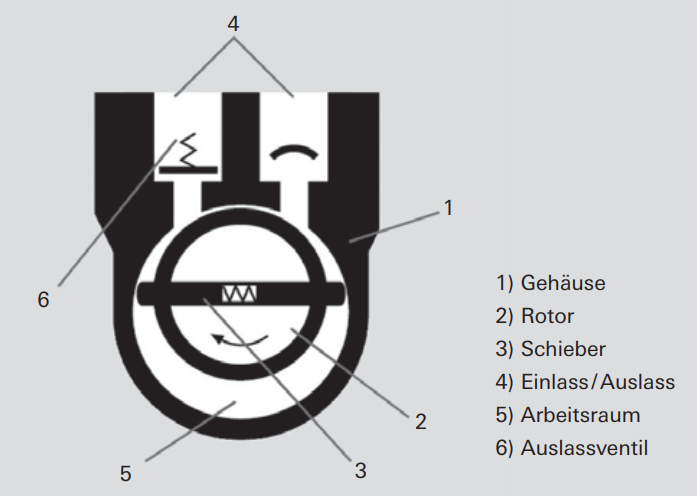
\includegraphics[width=0.6\textwidth]{Drehschieberpumpe.png}
        \caption{Schematische Abbildung deiner Drehschieberpuumpe.}
    \end{figure}

\subsubsection{Turbomolekularpumpe}
Turbomolekularpumpen sind kinetische Vakuumpumpen.
Sie sind Turbinenähnlich aufgebaut, innerhalb des Gehäuses sind mehrere Schichten abwechselnd mit Rotorscheiben und Statorscheiben besetzt.
Die Schaufeln der Schichten sind angewinkelt und zwischen Rotor und Strator spiegelverkehrt. 
Zur erzeugung eines Vakuums macht sich die Turbopumpe den Effekt der Adsorption zu nutze. Die Rotoren drehen sich während sich ein Molekül an denm Rotorblatt 
anheftet. Bei der Desorption hat das Molekül durch die angewinkelte Rotorscheibe und deren Rotation, einen Impuls, der bevorzugt weg vom Rezipienten zeigt.
Damit dieses Prinzip funktioniert, muss eine Molekulare Strömung herrschen, daher benötigt die Turbopumpe ein Vorvakuum. Zudem müssen die Rotorblätter ähnliche Geschwindigkeiten 
erreichen wie die Gasmoleküle, weshalb der Rotor sich mit bis zu 1500 Hz dreht.
Damit erreicht die Pumpe Drücke im Bereich des Hochvakuums \cite{Pfeiffer, S.83,84}.


\subsection{Vakuummessung}
\subsubsection{Pirani-Vakuummeter}
Das Pirani-Vakuumeter ist ein Wärmeleitungsvakuumeter. Es besteht aus einem Heizdraht in der Mitte eines Gehäuses.
Der Druck wird bestimmt, in dem die Wärmeleitfähigkeit des Gases zwischen Heizdraht und Gehäuse gemessen wird. 
Diese ist im Bereich von $10 mbar$ bis $10^{-4}\: mbar$ hauptschlich durch Stöße der Gasteilchen gegeben und verläuft liner zum Druck \cite{Pfeiffer, S.93,94}.


\subsubsection{Kaltkathoden-Ionisationsvakuumeter}
Bei desem Vakuumeter werden durch ein elektrisches Feld Elektronen aus der Kathode gelöst und in Richtung Anode beschleunigt.
Zwischen Kathode und Anode ionisieren die Elektronen durch Stöße die Gas-Teilchen, wodurch eine Gasentladung zustande kommt.
Der Gasentladungsstrom ist dann proportional zum Druck.
Das Kaltkathoden-Ionisationsvakuumeter kann für Druckbereiche unterhalb von $p = 10^{-2}\: mbar$ genutzt werden\cite{Pfeiffer, S.94}.

\subsubsection{Heißkathoden-Ionisationsvakuumeter}
Das Prinzip ist änhlich zum Kaltkathoden-Ionisationsvakuumeter, nur werden hier die Elektronen durch das Anlegen einer Spannung an einen Glühdrat und den dadurch provozierten 
Glühelektrischen Effekt erzeugt. Die Druckbestimmung erfolgt ebenfalls durch Ionisation der Gas-Teilchen\cite{Pfeiffer, S.94,95}.

\subsubsection{Piezo-Vakuumeter}
Das Piezo-Vakuumeter besteht aus einem Volumen mit Druck $p_0$, welches durch eine Membran von dem Volumen des Rezipienten mit $p_1$, getrennt ist.
Bei Druckunterschieden zwischen $p_0$ und $p_1$ wirkt eine Kraft auf die Oberfläche der Membran, wodurch diese gedehnt wird. In der Membran sind 
piesokristalle eindiffundiert, welche bei besagter Dehnung eine Spannung erzeugen, durch die auf den Druck im Rezipienten geschlossen werden kann.
Diese Art von Vakuumeter wird vorallem im Grobvakuum eingesetzt \cite{Pfeiffer, S.92}.
















